\subsection{Use Case for applying \cbc}
\label{sec:usecase} 

``Router'' use case exposes an example of a simple ``Router'' component with configured quality of service (QoS) management, which is used in telecommunication networks. In this use case Stakeholders have provided the system requirements (\autoref{tab:SR}) as a text document with semi-structured information and a simple component diagram (\autoref{fig:route}). 
\begin{figure}[!t]
\centering
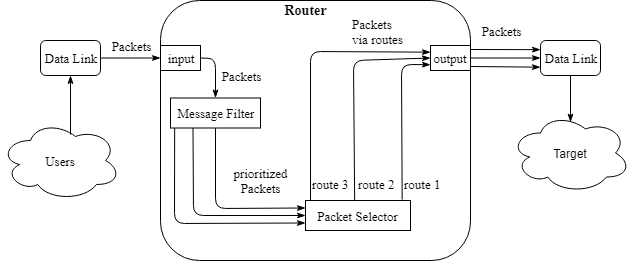
\includegraphics[width=3.5in]{use_case/router.png}
\caption{Diagram of the Router in the Network}
\label{fig:route}
\end{figure}

\begin{table}
	\centering
		\begin{tabular}{p{8cm}}
\small
\begin{center}
\textbf{\textit{System requirements.}}
\end{center}
``In communication system Data Link (DL) is usually used by several users. The users can proceed with different types of traffic. For better use of Data Link resources, traffic from diverse users can differ by priorities (depends on QoS and user's agreement). Depending on the priority, traffic should be forwarded along a certain route with a defined latency. For high priority packets the route shall be defined with the lowest latency. The lower priority of traffic, the higher latency the provided route has. Configuration input for Selector should be specified by QoS agreement of user.

Message Filter defines priority of packets and send them directly to Selector. 

Selector should:
\begin{itemize}
	\item receive packets from Message Filter;
  \item define a proper route, according to packet priority;
\end{itemize}

Packets shall be sent from Selector to Data Link using 3 routes.

All QoS policy is defined in Selector component. 

There are 3 data priorities: 
\begin{enumerate}
	\item High priority information - Selector should route such packets into 1st route only! 
  \item	Middle level priority - packets can be sent by Selector into 1st route , if the route is free; otherwise, traffic is transmitted into 2nd route;
  \item	Low priority - data can be sent in 3 routers, depends on which route is free at the moment.''
\end{enumerate}
\end{tabular}
	\caption{System Requirements Provided by Stakeholders}
	\label{tab:SR}
\end{table}

\normalsize 
\subsubsection{Requirements Structuring}
\label{sec:reqstruct}
Initial phase of development process is elicitation and analysis of requirements. We claim, that during analysis process \asp should be applied to the requirements in order to categorize them and form their structure. Considering further the ``Router'' use case, the following \asp can be assigned to the given requirements:\\

\small ``Req-1.	In communication system Data Link is usually used by several users.''

\normalsize[\textit{Mode aspect}] implies, that DL is in active state, when the users send traffic.\\

\small ``Req-2.	The users can proceed with different types of traffic.''

\normalsize [\textit{Signal aspect}] describes, that the packets have different types.\\

\small ``Req-3.	For better use of Data Link resources, traffic from diverse users can differ by priorities (depends on QoS in user's agreement).''

\normalsize [\textit{Signal aspect}] describes the traffic.\\

\small ``Req-4.	Depending on the priority, traffic should be forwarded along a certain route with a defined latency.'' 

\normalsize \begin{itemize}
	\item \textit{Parameter definition aspect} indicates, that priorities, routes and latency can be kept as re-useable parameters;
	\item \textit{Signal aspect} describes input for the routes;
	\item \textit{Functional aspect} describes the behavior of ``Packets Selector'';
	\item \textit{Temporal property aspect} shows, that the statement includes a condition;
\end{itemize}

The rest of the requirements should be analyzed and structured similarly.

After requirements have been categorized, the requirements engineer can proceed with the following inspection. First of all, he/she should check, if all requirements have \asp. Next, re-consider the requirements with more than 1 aspect in their categorization; it can mean, that such requirements are not precise enough. For example, the requirement ``Req-4'':\\

\small ``Req-4. Depending on the priority, traffic should be forwarded along a certain route with a defined latency.``

\normalsize
\begin{itemize}
	\item \textit{Parameter definition aspect}, 
	\item \textit{Signal aspect},
	\item \textit{Functional aspect}, 
	\item \textit{Temporal property aspect.}
\end{itemize}

It can be splitted into several requirements according to \asp categories:\\

For [\textit{Functional aspect}]:

\small
``Req-4.1.	 Selector should forward traffic along a certain route.''\\

\normalsize For [\textit{Parameter definition aspect}]:

\small
``Req-4.2.	 Every route operates with defined latency.''

``Req-4.3.	There are several (three) routes.''

``Req-4.4.	There are several priorities for traffic.''\\

\normalsize For [\textit{Signal aspect}]:

 \small ``Req-4.1.	Traffic is prioritized.''\\

\normalsize For [\textit{Temporal property aspect}]:

\small ``Req-4.2.	Traffic priority defines a route for traffic.''\\

\normalsize The ideal case is when every requirement has only one aspect, but in real project requirements categories usually overlap each other. Therefore, the number of \asp attached to a requirement should tend to be minimized.

After applying this method also to the other requirements, we have obtained the following structure of requirement, presented in \autoref{tab:structuredHLR}.

\begin{table*}
	\centering
		\begin{tabular}{| p{11cm}  | p{6cm} |}
			\small ``Req-1.	 In communication system Data Link is usually used by several users.'' &	[\textit{Mode aspect}]\\
``Req-2.	The users can proceed with different types of traffic.'' & [\textit{Signal aspect}]\\	
``Req-3.	For better use of Data Link resources, traffic from diverse users can differ by priorities (depends on QoS in user's agreement).'' & [\textit{Signal aspect}] \\
``Req-4.1	 Selector should forward traffic along a certain route.''& [\textit{Functional aspect}]\\ 
``Req-4.2	Every route operates with defined latency.'' & [\textit{Parameter definition aspect}]\\		
``Req-4.3	There are several (three) routes.'' & [\textit{Parameter definition aspect}] \\
``Req-4.4 There are several priorities for traffic.'' & [\textit{Parameter definition aspect}]\\
``Req-4.5	Traffic is prioritized.'' & [\textit{Signal aspect}] \\
``Req-4.6	Traffic priority defines a route for traffic.'' & [\textit{Temporal property aspect}] 	\\
``Req-5.	For high priority packets the route shall be defined with the lowest latency.'' & [\textit{Temporal property aspect}] \\
``Req-6.	The lower priority of traffic, the higher latency the provided route has.'' & [\textit{Temporal property aspect}] \\
``Req-7.	Configuration input for Selector should be specified by QoS agreement of user.'' & [\textit{Signal aspect}] \\
``Req-8.1	Message Filter defines priority of packets.'' & [\textit{Functional aspect}] \\	
``Req-8.2 Message Filter sends packets directly to Selector.'' &  [\textit{Functional aspect}] \\
``Req-9.1	Selector should receive packets from Message Filter.'' & [\textit{Functional aspect}] \\
``Req-9.2	Selector should define a proper route, according to packet priority.'' & [\textit{Functional aspect and Temporal property aspect}]\\
``Req-10.1	Selector shall send packets to Data Link.'' & [\textit{Functional aspect and Signal aspect}] \\
``Req-10.2	Selector shall use 3 routes for packets sending to Data Link.'' & [\textit{Functional aspect}] \\
``Req-10.3	There are 3 routes for sending packets from Selector to Data Link.'' & [\textit{Parameter definition aspect}] \\
``Req-11	All QoS policy is defined in Selector component.'' & [\textit{Functional aspect}] \\
``Req-12.1	There are 3 data priorities.'' & [\textit{Parameter definition aspect}] \\
``Req-12.2.	High priority information - Selector should route such packets into 1st route only!'' & 
[\textit{Temporal property aspect}] \\
``Req-12.3.	Middle level priority - packets can be sent by Selector into 1st route , if the route is free; otherwise, traffic is transmitted into 2nd route.'' & [\textit{Temporal property aspect}] \\
``Req-12.4.	Low priority - data can be sent in 3 routers, depends on which route is free at the moment.'' & [\textit{Temporal property aspect}] \\
		\end{tabular}
	\caption{Structured Requirements with Attached Aspects}
	\label{tab:structuredHLR}
\end{table*}

\normalsize
Now we have more consistent high-level requirements (HLR) in comparison with the requirements initially provided by the stakeholder. That means, the requirements are better structured, more precise and less complex. These characteristics rise quality of the requirements. Therefore, it is easier to work with such requirements during development phase or review process.

These structured HLR now can be an input for system design process. Developers can also analyze the requirements and provide additional requirements, which were inferred from HLR. For this purpose, there exists a \textit{Design Choice aspect}. This aspect indicates, that changes in requirements have been done by developers team. Example of such requirement is provided:

\small''Req-13.  Packets follow the Ethernet standard.''

\normalsize the requirement now has two \asp [\textit{Signal aspect} and \textit{\textbf{Design Choice aspect}}]. 


\normalsize \subsubsection{Requirements Review}
\textit{Aspects} support also requirements review process. Every \textit{aspect} provides a check-list specified for respective category of requirement. This feature serves for more rigorous review of the requirements instead of a general check. More over, different \asp imply different activities of requirements checking. As an example from the use case, to inspect Req-10.2: \\

\small ``Req-10.2.  Selector shall use 3 routes for packets sending to Data Link.'' 

\normalsize [\textit{Functional aspect}], here reviewer checks correctness of algorithms implemented within this requirement. However, the same check is useless for Req-4.3: \\

\small ``Req-4.3.  There are several (three) routes.'' 

\normalsize ,which is defined by [\textit{Parameter definition aspect}].\\

Working with HLR structured by \asp, the reviewer can trigger the following revision:
\begin{itemize}
	\item whether \textit{aspects} have been applied to each requirement,
  \item whether the \textit{aspects} match appropriately with the considered requirements (the reviewer can propose additional \asp or make changes in the ones already attached),
	\item whether all \asp check-lists give successful outcomes.
\end{itemize}
